\documentclass[a4paper, 10pt, danish, final]{article}
\usepackage{bonde}

\def\mytitle{Dataanalyse 2010}
\def\mysubtitle{Aflevering af ugeopgave 1}
\def\myauthor{Ulrik Bonde}
\def\mymail{\mailto{bonde@diku.dk}}
\def\mydate{\today}
\def\repository{\url{http://github.com/bonde/dataanalyse}}

\title{\mytitle}
\subtitle{\mysubtitle}

\author{\myauthor{} - \mymail}
\date{\mydate}

\hypersetup{
colorlinks,%
citecolor=black,%
filecolor=black,%
linkcolor=black,%
urlcolor=black,%
bookmarksopen=false,
pdftitle={\mytitle{} - \mysubtitle},
pdfauthor={\myauthor}
}

\begin{document}
\maketitle

\subsection*{Spørgsmål 1}
Vi har givet signalet $g[x]=[1_{\centerdot}, 2, 3, 2, 1, 0, -1, -2]$ og
filteret $f[x]=[1_{\centerdot}, -1]$. Prikken indikerer starten af en
periode. Vi vil gerne konstruere $g_e(x)$ og $f_e(x)$. I henhold til
\citep[s. 15]{soereninout} har vi at $A = 2$ og $B = 8$, dvs. blot
længden af hhv. filteret og signalet.

\begin{equation}
    f_e(x) = \left\{ \begin{array}{l l l}
        f(x) & \mbox{hvis} & 0 \leq x \leq A - 1\\
        0 & \mbox{hvis} & A \leq x \leq M - 1
    \end{array}\right.
\end{equation}

\begin{equation}
    g_e(x) = \left\{ \begin{array}{l l l}
        g(x) & \mbox{hvis} & 0 \leq x \leq A - 1\\
        0 & \mbox{hvis} & A \leq x \leq M - 1
    \end{array}\right.
\end{equation}
hvor
\begin{align}
    M & \geq A + B - 1\nonumber\\
    & \geq  2 + 8 - 1\\
    & \geq  9\nonumber
\end{align}
$M$ er ligeledes den minimale længde af foldningen.

Ved at bruge ovenstående på de originale signaler får vi
\begin{equation}
    f_e(x) = [1_{\centerdot}, -1, 0, 0, 0, 0, 0, 0, 0]
\end{equation}
og
\begin{equation}
    g_e(x) = [1_{\centerdot}, 2, 3, 2, 1, 0, -1, -2, 0]
\end{equation}

Vi spejler signalet $g_e(x)$ og får $g'_e(x) = [0, -2, -1, 0, 1, 2, 3,
2, 1_{\centerdot}]$. Resultatet af foldningen $(f \star g)(x) = h[x] =
[1_\centerdot, 1, 1, -1, -1, -1, -1, -1, 2]$ af længde 9.

I tabel \ref{tabel_folding} ses hvorledes foldingen
\emph{kan} udledes. I praksis finder jeg det forvirrende at spejle
signalet. Da foldningen $(f \star g)(x) = (g \star f)(x)$ tager jeg
udgangspunkt i at man kan spejle filteret og lade dette køre over
signalet.

\begin{table}[t]
    \begin{equation}
        \rowcolors[]{1}{gray!20}{gray!10}
        \begin{array}{c|cccccccccccc|c}
            x & 0 & -2 & -1 & 0 & 1 & 2 & 3 & 2 & 1_{\centerdot} & 0 & -2 & \cdots & h(x) = \sum_{\alpha \in \mathcal{N}}f(\alpha)g(x - \alpha)\\\hline
            0&&&&&&&&&1_\centerdot & -1 &&& (1\cdot 1) + (-1 \cdot 0) = 1\\
            1&&&&&&&&1_\centerdot & -1 &&&& (1\cdot 2) + (-1 \cdot 1) = 1\\
            2&&&&&&&1_\centerdot & -1 &&&&& 3 - 2 = 1\\
            3&&&&&&1_\centerdot & -1 &&&&&& 2 - 3 = -1\\
            4&&&&&1_\centerdot & -1 &&&&&&& 1 - 2 = -1\\
            5&&&&1_\centerdot & -1 &&&&&&&& 0 - 1 = -1\\
            6&&&1_\centerdot & -1 &&&&&&&&& -1 + 0 = -1\\
            7&&1_\centerdot & -1 &&&&&&&&&& -2 + 1 = -1\\
            8&1_\centerdot & -1 &&&&&&&&&&& 0 + -(-2) = 2
        \end{array}\nonumber
    \end{equation}
    \caption{Udregning af foldingen $(f \star g)(x)$. I tabellen ses
    hvordan filteret rykker et trin til venstre for hver iteration, men
    egentlig er det selve signalet som rykker til højre. Vi ser at
    foldningen resulterer i signalet $h[x] = [1_\centerdot, 1, 1, -1,
    -1, -1, -1, -1,
    2]$.}
    \label{tabel_folding}
\end{table}

\subsection*{Spørgsmål 2}
Givet signalet $f[x] = [1, 0, 1, 0]$ ønsker vi at beregne
Fouriertransformationen. En meget naiv løsning er blevet implementeret i
MATLAB som kontrol. Denne følger definitionen givet i \citep[ligning
2.14, s. 16]{soereninout}. Funktionen \texttt{DANaiveFourier.m} er
vedlagt som bilag.

For $u = 0$ har vi at $e^{-2\pi i \cdot 0/4} = e^{0} = 1$ for alle
værdier af $x$
\begin{equation}
    \mathcal{F}(0) = \frac{1}{4}(1 + 0 + 1 + 0) = \frac{1}{2}
\end{equation}

For $u = 1$ har vi
\begin{align}
    x = 0 & : e^{-2\pi i \cdot 1 \cdot 0/4} = 1\\
    x = 1 & : e^{-2\pi i \cdot 1 \cdot 1/4} = i\\
    x = 2 & : e^{-2\pi i \cdot 1 \cdot 2/4} = -1\\
    x = 3 & : e^{-2\pi i \cdot 1 \cdot 3/4} = -i
\end{align}
og derved
\begin{equation}
    \mathcal{F}(1) = \frac{1}{4}(1 + 0 - 1 + 0) = 0
\end{equation}

For $u = 2$ har vi
\begin{align}
    x = 0 & : e^{-2\pi i \cdot 2 \cdot 0/4} = 1\\
    x = 1 & : e^{-2\pi i \cdot 2 \cdot 1/4} = -1\\
    x = 2 & : e^{-2\pi i \cdot 2 \cdot 2/4} = 1\\
    x = 3 & : e^{-2\pi i \cdot 2 \cdot 3/4} = -1
\end{align}
og får derfor
\begin{equation}
    \mathcal{F}(2) = \frac{1}{4}(1 + 0 + 1 + 0) = \frac{1}{2}
\end{equation}

Endelig for $u = 3$ har vi
\begin{align}
    x = 0 & : e^{-2\pi i \cdot 3 \cdot 0/4} = 1\\
    x = 1 & : e^{-2\pi i \cdot 3 \cdot 1/4} = -i\\
    x = 2 & : e^{-2\pi i \cdot 3 \cdot 2/4} = -1\\
    x = 3 & : e^{-2\pi i \cdot 3 \cdot 3/4} = i
\end{align}
og
\begin{equation}
    \mathcal{F}(3) = \frac{1}{4}(1 + 0 - 1 + 0) = 0
\end{equation}

\begin{lstlisting}[caption={Fouriertransformation i MATLAB
    (kommandoprompt)}, captionpos=b,
    label={fft_matlab}, float=t, numbers=none]
>> fft([1 0 1 0])

ans =

     2     0     2     0

\end{lstlisting}

Resultatet er altså at $\mathcal{F} = [\frac{1}{2}, 0, \frac{1}{2}, 0]$.
Dog --- som vist i kodeboks \ref{fft_matlab} --- findes et andet
resultat hvis vi bruger MATLABs indbyggede funktion \texttt{fft}. Dog
ses det let at man i MATLAB \emph{ikke} dividerer summen
$\sum_{x=0}^{N - 1}f(x)e^{-2\pi iux}$ med $N$ når
transformationen beregnes. Et hurtigt opslag i MATLABs dokumentation
bekræfter dette. Vi ville også få samme resultat hvis vi undlod at
dividere med $N$.

\subsection*{Spørgsmål 3}

Vi betragter nu frekvenssignalet
\begin{equation}
    \mathbf{F}[u] = \left\{ \begin{array}{l l l}
        A & \mbox{hvis} & u = 1\\
        B & \mbox{hvis} & u = T + 1\\
        B & \mbox{hvis} & u = N - T + 1\\
        0 & \mbox{ellers} &
    \end{array}\right.
\end{equation}
med $N = 64$. At vi har et frekvenssignal betyder at vi betragter
Fouriertransformationen af et signal. Det er let at se at kun tre indeks
i signalet vil have en værdi. Hvis vi sætter $A = 10, B = 20$ og
$T = 4$ får vi frekvenssignalet vist i figur \ref{freq_10_20_4} og det
tilsvarende signal i tidsdomænet i figur \ref{time_10_20_4}. Signalet i
tidsdomænet er frembragt ved invers Fouriertransformation af
$\mathbf{F}[u]$ som vist i kodeboks \ref{ifft_matlab}.

\begin{figure}[!h]
    \centering
    \subfloat[Signal i
    frekvensdomænet]{\label{freq_10_20_4}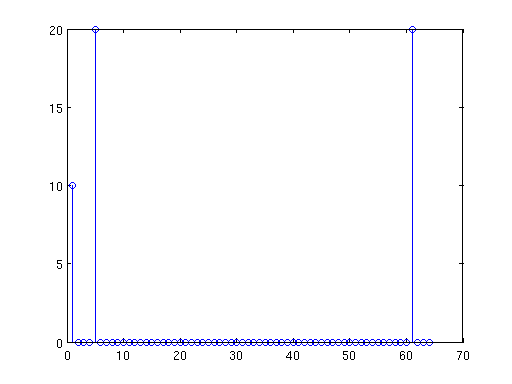
\includegraphics[angle=0,width=0.45\textwidth]{images/freq_10_20_4}\hspace{1em}}
    \subfloat[Signal i tidsdomænet]{\label{time_10_20_4}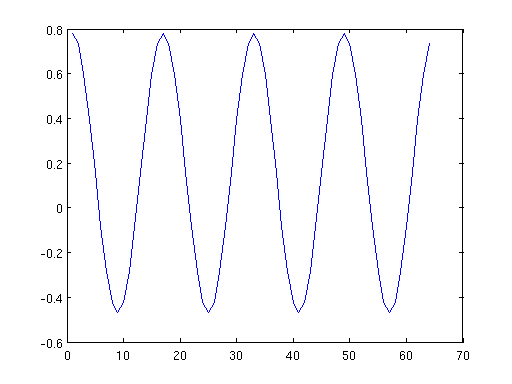
\includegraphics[angle=0,width=0.45\textwidth]{images/time_10_20_4}}
    \caption[]{To forskellige repræsentationer af signalet genereret ved
    at sætte $A = 10, B = 20$ og $T = 4$.}
    \label{signal_10_20_4}
\end{figure}

Signalet vist i figur \ref{freq_10_20_4} har origo i 1 og er derfor
symmetrisk omkring dette indeks. Derved er frekvenssignalet periodisk.
Man kan benytte den indbyggede funktion \texttt{fftshift} til at
``flytte'' rundt i signalet således at origo er i midten. Egentlig tager
man bare og bytter den ene halvdel af signalet med den anden, dvs.
$F(1:N/2)$ flyttes til $F(N/2+1:end)$ og omvendt.

Man kan uden videre ræsonnere sig frem til at parameteren $T$ har noget
at gøre med frekvensen af signalet i tidsdomænet. Dog er det interessant
at se, at $T$ angiver antallet af maksima, dvs. svingninger, i signalet.
Dette er illustreret i figur \ref{signal_10_20_8_16}.

På samme måde ved vi at vi har middelværdien af signalet i origo og
parameteren $A$ regulerer denne. I figur \ref{signal_10_20_4} havde vi
sat $A = 10$ og vi ser at midten af sinusbølgen ``har midtpunkt''
(horisontalt) over x-aksen. Dette lyder forvirrende og det er derfor
illustreret i figur \ref{signal_0_50_4}. Her set det, at når vi sætter $A = 0$ vil
sinusbølgen have symmetriakse i på x-aksen. Endvidere viser figur
\ref{signal_0_50_4} at parameteren $B$ er sinusbølgens amplitude.

\begin{figure}[!h]
    \centering
    \subfloat[Signal i frekvensdomænet]{\label{freq_10_20_8}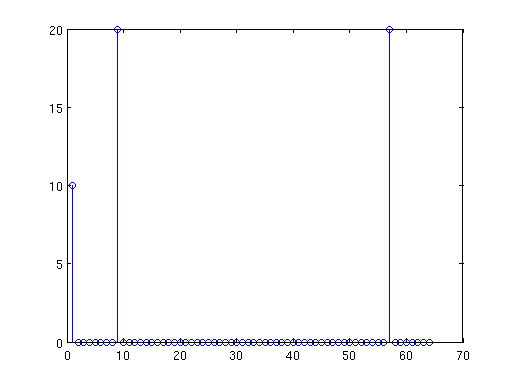
\includegraphics[angle=0,width=0.45\textwidth]{images/freq_10_20_8}\hspace{1em}}
    \subfloat[Signal i tidsdomænet]{\label{time_10_20_8}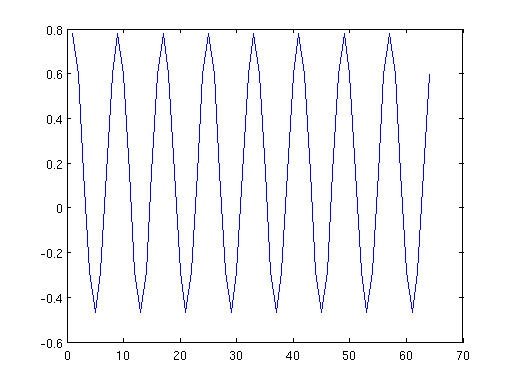
\includegraphics[angle=0,width=0.45\textwidth]{images/time_10_20_8}}\\
    \subfloat[Signal i frekvensdomænet]{\label{freq_10_20_16}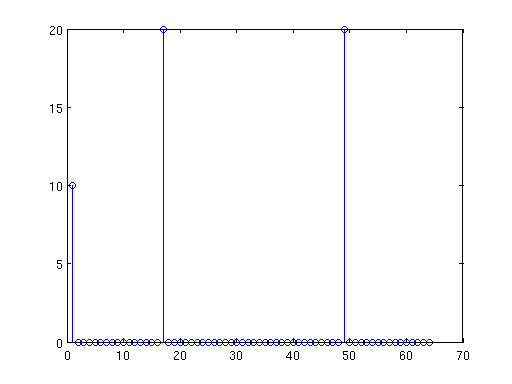
\includegraphics[angle=0,width=0.45\textwidth]{images/freq_10_20_16}\hspace{1em}}
    \subfloat[Signal i tidsdomænet]{\label{time_10_20_16}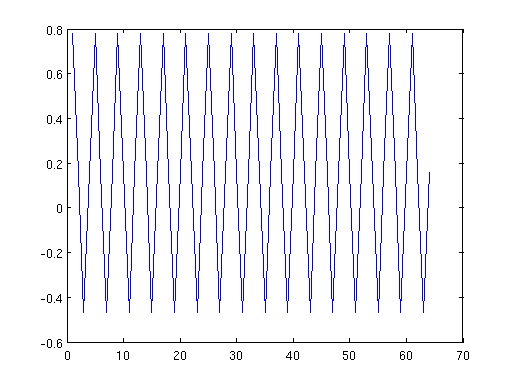
\includegraphics[angle=0,width=0.45\textwidth]{images/time_10_20_16}}
    \caption[]{
    \textbf{Øverst:} Signal genereret ved $A = 10, B = 20$ og $T = 8$
    \textbf{Nederst:} Signal genereret ved $A = 10, B = 20$ og $T = 16$
    Bemærk, at når impulserne givet ved $B$ flytter sig længere væk fra
    origo, så stiger frekvensen i signalet. Dette er et godt eksempel på
    at lave frekvenser findes omkring origo, mens høje frekvenser findes
    i yderpunkterne.
    }
    \label{signal_10_20_8_16}
\end{figure}

\begin{figure}[!h]
    \centering
    \subfloat[Signal i frekvensdomænet]{\label{freq_0_50_4}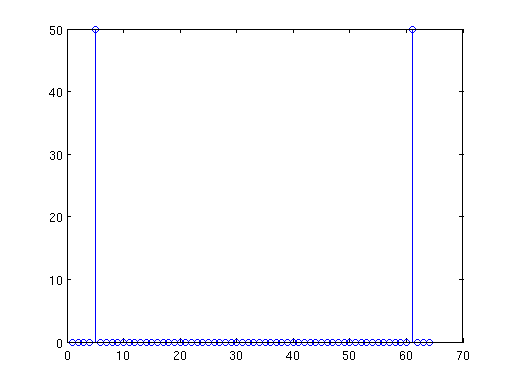
\includegraphics[angle=0,width=0.45\textwidth]{images/freq_0_50_4}\hspace{1em}}
    \subfloat[Signal i tidsdomænet]{\label{time_0_50_4}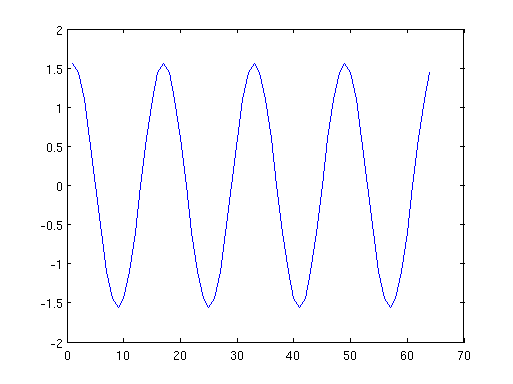
\includegraphics[angle=0,width=0.45\textwidth]{images/time_0_50_4}}
    \caption[]{To forskellige repræsentationer af signalet genereret ved
    at sætte $A = 0, B = 50$ og $T = 4$. Her skal tallene på y-aksen
    bemærkes. I tidsdomænet har vi større amplitude og sinusbølgen har
    midte på x-aksen.}
    \label{signal_0_50_4}
\end{figure}

\begin{lstlisting}[caption={Invers Fouriertransformation i MATLAB og
    plot af signaler
    (kommandoprompt)}, captionpos=b,
    label={ifft_matlab}, float=t]
>> close all;                               % Good meassure
>> A = 10; B = 20; T = 4;                   % Init parameters
>> F = DAImpulses(A, B, T);                 % Create impulses
>> f = real(ifft(F));                       % Inverse Fourier transform
>> figure(1); stem(F);                      % Plot impulses
>> figure(2); plot(f);                      % Plot inverse transform

\end{lstlisting}


%%%%%%%%%%%%%%%%%%%%%%%%%%%%%%%%%%%%%%%%%%%%%%%%%%%%%%%%%%%%%%%%%%%%
% Formal stuff

\bibliographystyle{abbrvnat}
\bibliography{bibliography}
%\addcontentsline{toc}{chapter}{Litteratur}

\appendix
\lstset{language=Matlab, basicstyle=\scriptsize,
    showstringspaces=false, numbers=left, stepnumber=1,
    numberstyle=\tiny, frame=none}
\section{Kildekode}
Kildekoden er tilgængelig i mit git-repository på \repository{}. Bemærk
at prefikset \texttt{DA} står for ``DataAnalyse'' og blot er til for at
undgå eventuelle sammenstød med indbyggede funktioner i MATLAB.

\subsection{DANaiveFourier.m}
\lstinputlisting{../src/DANaiveFourier.m}

\subsection{DAImpulses.m}
\lstinputlisting{../src/DAImpulses.m}

\end{document}

% vim: set tw=72 spell spelllang=da:
